\documentclass[11pt,a4paper]{article}
\usepackage[utf8]{inputenc}
\usepackage[margin=2.5cm]{geometry}
\usepackage{graphicx}
\usepackage{float}
\usepackage{xcolor}
\usepackage{listings}
\usepackage{hyperref}
\usepackage{graphicx}

\graphicspath{ {./images/} }

\title{Behind the Scenes}
\author{Carlo Ramponi}
\date{22 April 2022}

\definecolor{codegreen}{rgb}{0,0.6,0}
\definecolor{codegray}{rgb}{0.5,0.5,0.5}
\definecolor{codepurple}{rgb}{0.58,0,0.82}
\definecolor{backcolour}{rgb}{0.95,0.95,0.92}

\lstdefinestyle{mystyle}{
    backgroundcolor=\color{backcolour},   
    commentstyle=\color{codegreen},
    keywordstyle=\color{magenta},
    numberstyle=\tiny\color{codegray},
    stringstyle=\color{codepurple},
    basicstyle=\ttfamily\footnotesize,
    breakatwhitespace=false,         
    breaklines=true,                 
    captionpos=b,                    
    keepspaces=true,                 
    numbers=left,                    
    numbersep=5pt,                  
    showspaces=false,                
    showstringspaces=false,
    showtabs=false,                  
    tabsize=2
}

\lstset{style=mystyle}

\begin{document}
\begin{titlepage}

\centering
    \vfill
    \vskip3cm
    \Large Department of Information Engineering and Computer Science
    \vskip0.5cm
    \Large (DISI)
    \vskip2cm
    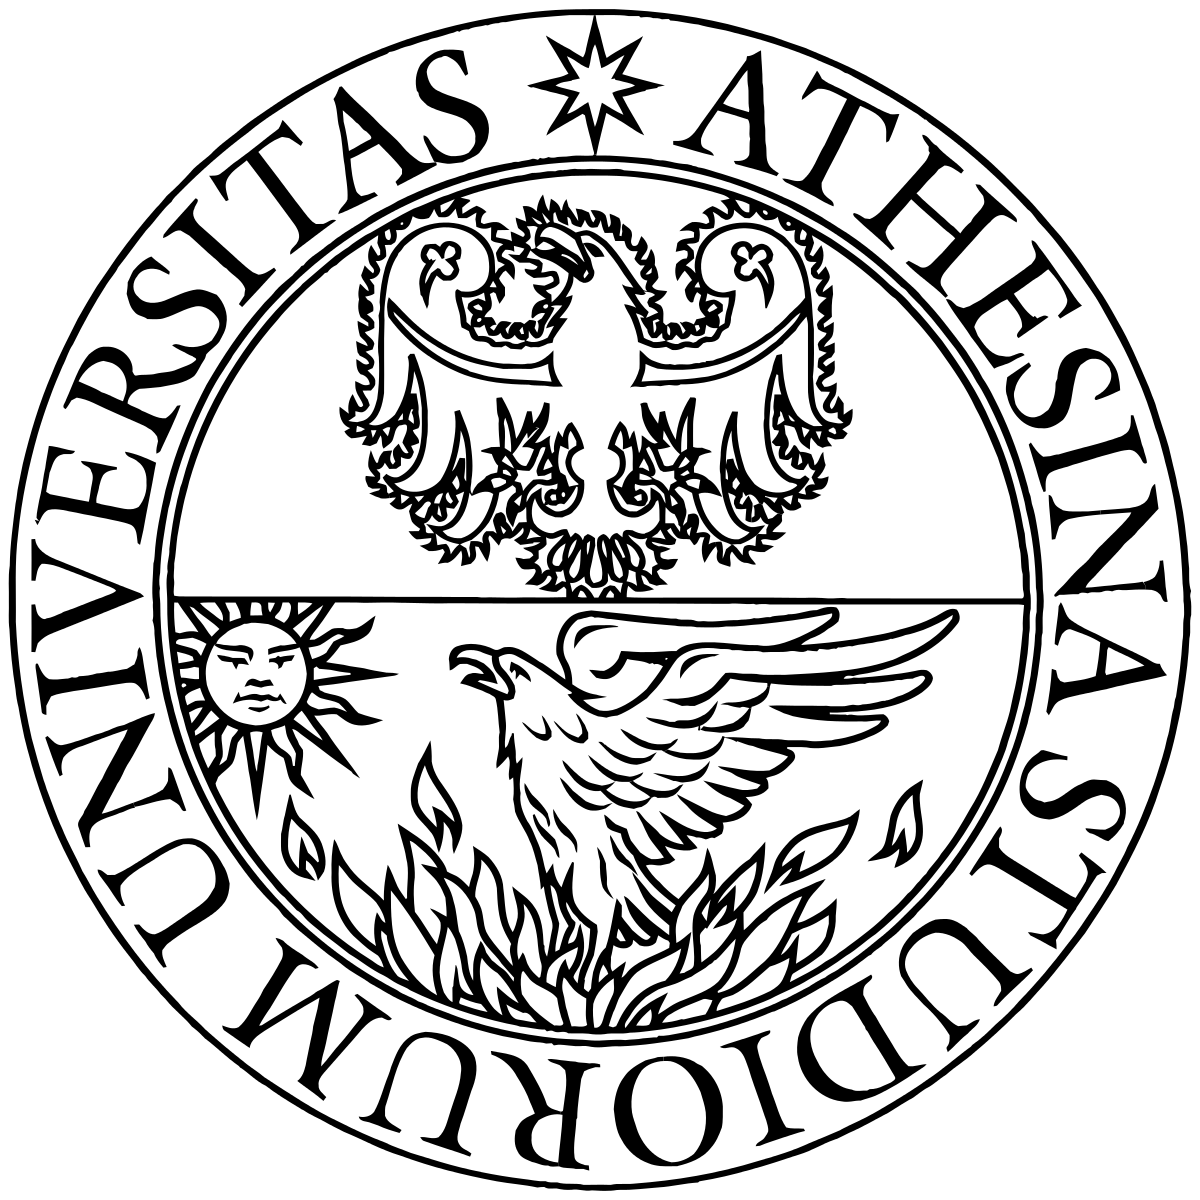
\includegraphics[width=8cm]{images/logo_unitn.png}
    \vskip2cm
    \textbf{\Large Network Security - A.Y. 2021/2022}
    \vskip2cm
    \textbf{\LARGE DNS}
    \vskip0.2cm
    \textbf{\LARGE Cache poisoning and Kaminsky attack}
    \vskip4cm
    \Large Carlo Ramponi, Luca De Menego, Matteo Zanotto
    \vfill

\end{titlepage}

\clearpage

\tableofcontents

\clearpage

\section{DNS specification}

\subsection{What is the DNS}

The \emph{Domain Name System} is a fundamental Internet service that maps human readable host names, such as \texttt{disi.unitn.com}, to IP addresses, such as \texttt{193.205.194.4}, that can actually be used by machines in networking.

\noindent
More generally, the DNS was developed to provide a consistent name space for referring to internet resources such as host domain names or mailboxes.

\noindent
It defines standard formats for representing the resource data and for methods to query the database.

\hfill \break
\noindent
The DNS was developed with scalability in mind to adapt to the increasing sheer size of internet data and usage: it is implemented in a distributed hierarchical manner as a tree structure, where more fine grained information about the resources is accessed by walking down a delegation mechanism.

\noindent
Additionally, local caching is applied to improve the performances: already known information is stored so it can be served directly without repeating queries.

\subsection{Typical DNS messages flow}
DNS queries typically follow a redirect flow between various name servers along the hierarchy until the resource is resolved. This is because each name server either answers the question posed in the query or refers the requester to another set of name servers when it is not able to resolve the query.

\hfill \break
\noindent
In a typical name resolution scenario, a DNS query will be generated by the client on the browser when trying to connect to a domain. The query will be received by a DNS recursive resolver, which will handle the query until a final response to return to the client. Assuming caches are empty, the recursive server will contact a root name server at the top of the hierarchy which will return a set of addresses for top level domain (TLD) name servers responsible for the input domain name. TLD name servers maintain information on domains that share the same domain extension, such as \texttt{.com}, \texttt{.it}, \texttt{.net} etc.

\noindent
The resolver will redirect the query to a top level domain server which will return the address of an authoritative name server: this is the final step of the name resolution as the authoritative server contains the specific information about the input domain address, it will not redirect the query to another name server.

\noindent
Once the resolver receives the answer from the authoritative name server the domain name is resolved to an IP address to which the client can finally connect.

\hfill \break
\noindent
Each interaction between the recursive resolver and the other name servers is identified by a query ID, that is generated by the resolver and is required to have the same value for both question and answer messages. This is a lightweight authentication mechanism that allows a recursive resolver to actually know that it is receiving a reply from a name server about the question it has sent. Responses that don't match the query ID will be discarded by the resolver, while legitimate responses are stored in the cache.

\subsection{DNS messages format}
A DNS packet is structured as a message with an header containing a set of always present fixed fields and a four section data content.

\hfill \break
\noindent
The header fields contain the 16 bit query ID, a flag for signaling the packet is a question or an answer, an opcode that identifies the type of the dns message, a flag for signaling recursion between name servers is desired in the name resolution process, a flag signaling the answer comes from an authoritative name server. Then there are a set of numbers that indicate the number of entries and authorities in the question or in the response. There are also fields for error handling.

\hfill \break
\noindent
The data content differs depending if it is a question or an answer but is generally structured in four sections for question data, answer data, authority data and additional data. 
In a question message there would be a \texttt{qname} field for the domain that needs to be resolved, a \texttt{qtype} field for the type of query (which is typically A for host addresses, NS for name server addresses, MX for mail servers) and a \texttt{qclass} field that specifies the query class, almost always with value IN as it refers to internet queries.

\noindent
An answer message will contain different data in the answer section depending on the type of resource that is returned. For example, in case of a domain name resolution with a \texttt{A} type it will contain the domain name, the IP address and the time to live of the information, while a redirection to another name server will contain a \texttt{NS} type answer with the name of the name server in the authority section together with an \texttt{A} type answer for the address of the name server in the additional information.

\hfill \break
\noindent
A DNS message is typically carried over a UDP packet for the fast performance requirements of the service.

\subsection{Resources representation}
All DNS data is stored in a core data structure called Resource Record (RR) which is internally composed of a series of fields and is identified by a name.

\hfill \break
\noindent
The fields of resource record are:
\begin{itemize}
\item Type, which specifies the abstract type of the resource in this resource record. The most common types are \texttt{A} for domain addresses, \texttt{NS} for name servers of a domain, \texttt{SOA} for authority information and \texttt{MX} for mail exchanges.
\item Class, for the protocol that it refers to, almost always with value \texttt{IN} for internet.
\item Rdata, for type and class depending data of the resource record. For example, in case of an A type resource record, it will be an IP address while for an NS resource record it will be a domain name.
\item TTL, the time to live of the information on the cache
\item Owner, often implicit
\end{itemize}

\hfill \break
\noindent
Since DNS resolvers query for a name, class and type, they are inherently querying for resource records.

\section{DNS implementation: Bind}

\subsection{Bind configuration}

\subsection{Zone files}

\section{Laboratory introduction}

\subsection{Katharà}

\subsection{Laboratory network topology}
\subsection{DNSSEC}
\begin{figure}[h]
  \centering
  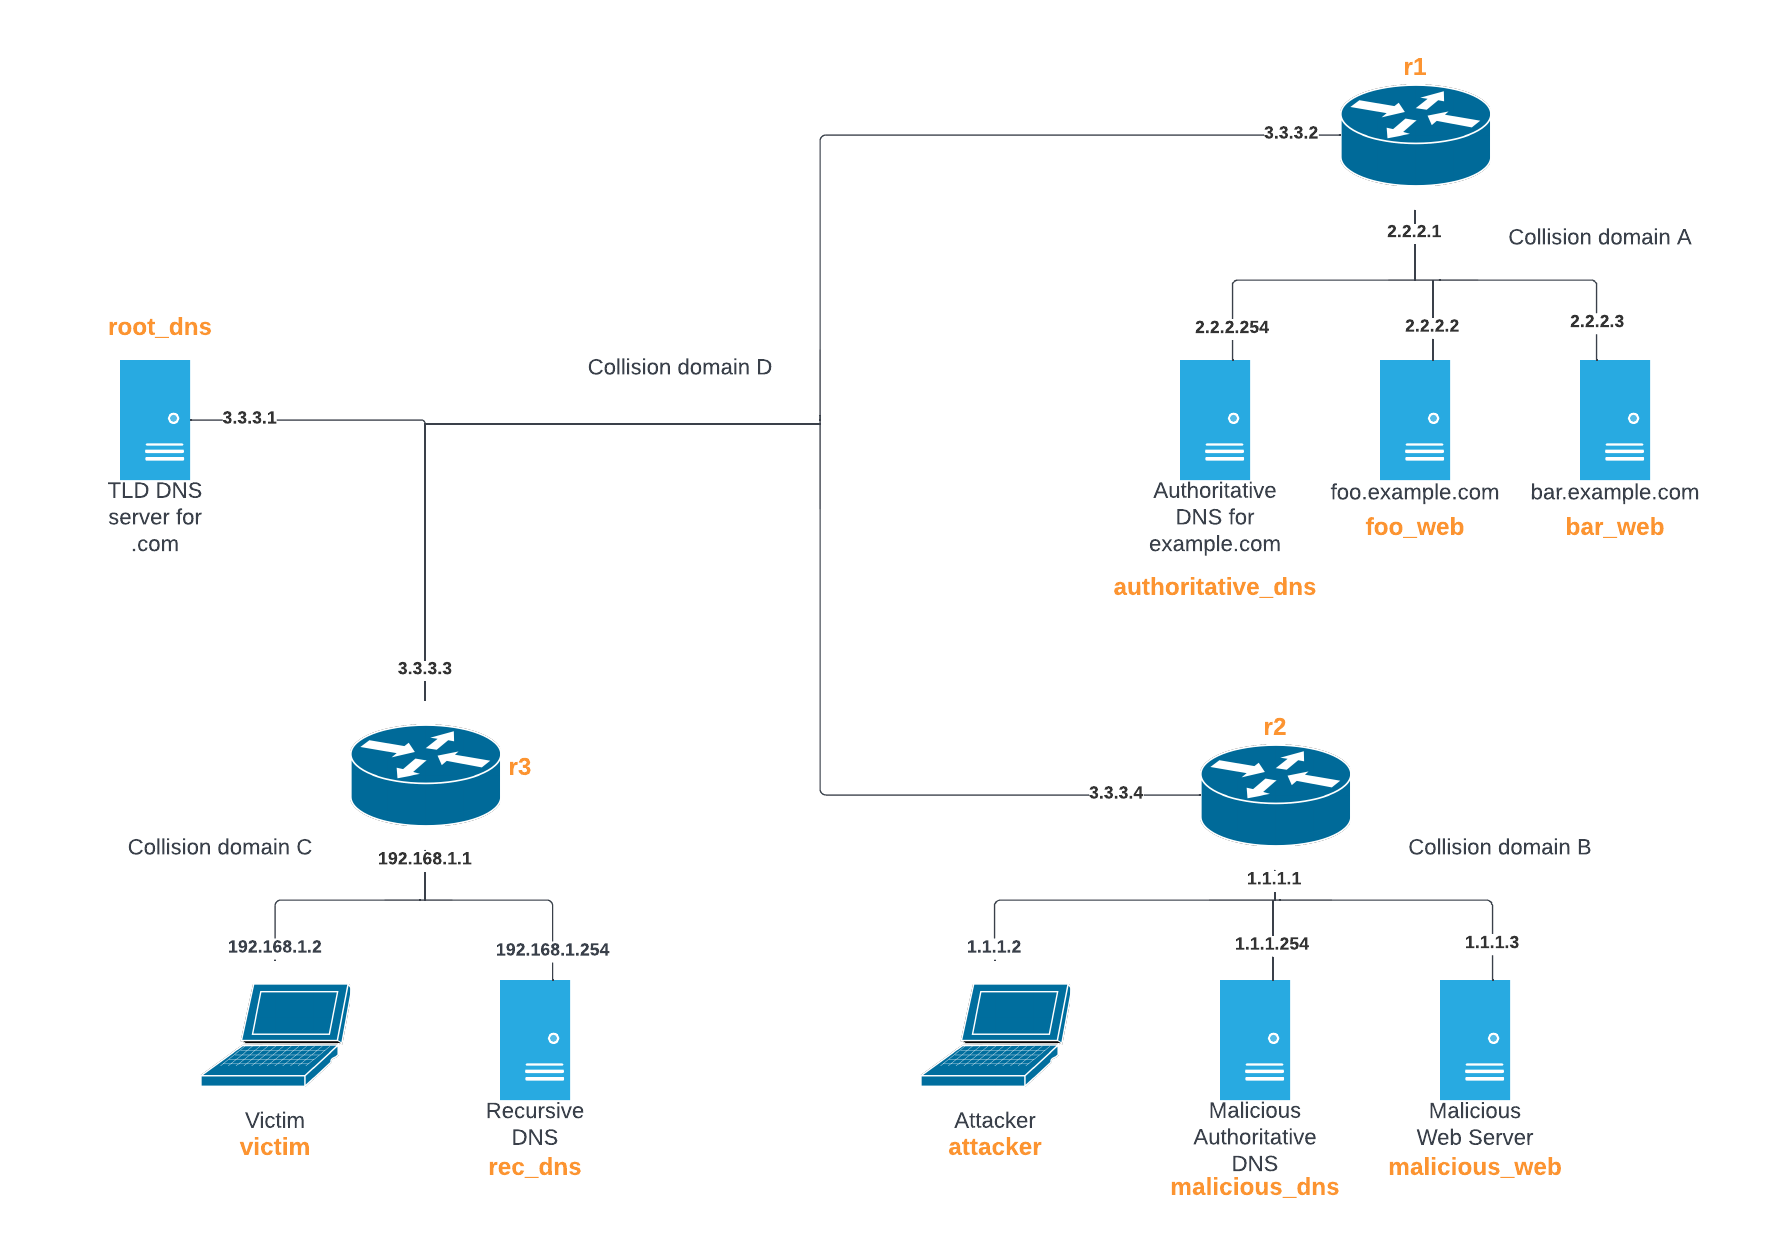
\includegraphics[scale=0.56]{network-topology.png}
  \caption{Laboratory network topology}
\end{figure}

\section{Final considerations}

\subsection{Performing the attack nowadays}

\subsection{DNSSEC}

\end{document}